\thispagestyle{endchapter}

\begin{tcolorbox}

\vspace{80pt}
	\lettrine{T}{he} weekend after the expedition van headed home, a small Slovene /
English team went back down \passage{M2} armed with an enormous drill \&
battery. With 6 shot holes they blew their way through the rift, to the
head of a short pitch.

This was returned to in October 2008, and dropped - all the new finds in
\passage{M2} being surveyed at the same time. The new pushing front is
another, almost impenetrable rift, and a climb up into a series of tight
phreatic passage. The survey data indicates that \passage{M2} itself is
trending away from \passage{Captain Kangaroo}.

During the expedition a
major error was discovered in our survey data - namely that the wrong
\passage{M2} entrance (there are two, separated by 25 m horizontal) was
connected into the surface survey. This caused a jump in the position of
the bottom of \passage{M2}, taking it further from \passage{Vrtnarija}.

With the corrected data, our closest approach is now 23 m between the
large chamber found below \passage{Cheesecake} and the confluence at the end of
\emph{M2}.

\end{tcolorbox} 
	\backgroundsetup{	scale=1,
					color=black,
					opacity=1,
					angle=0,
					contents={%
							  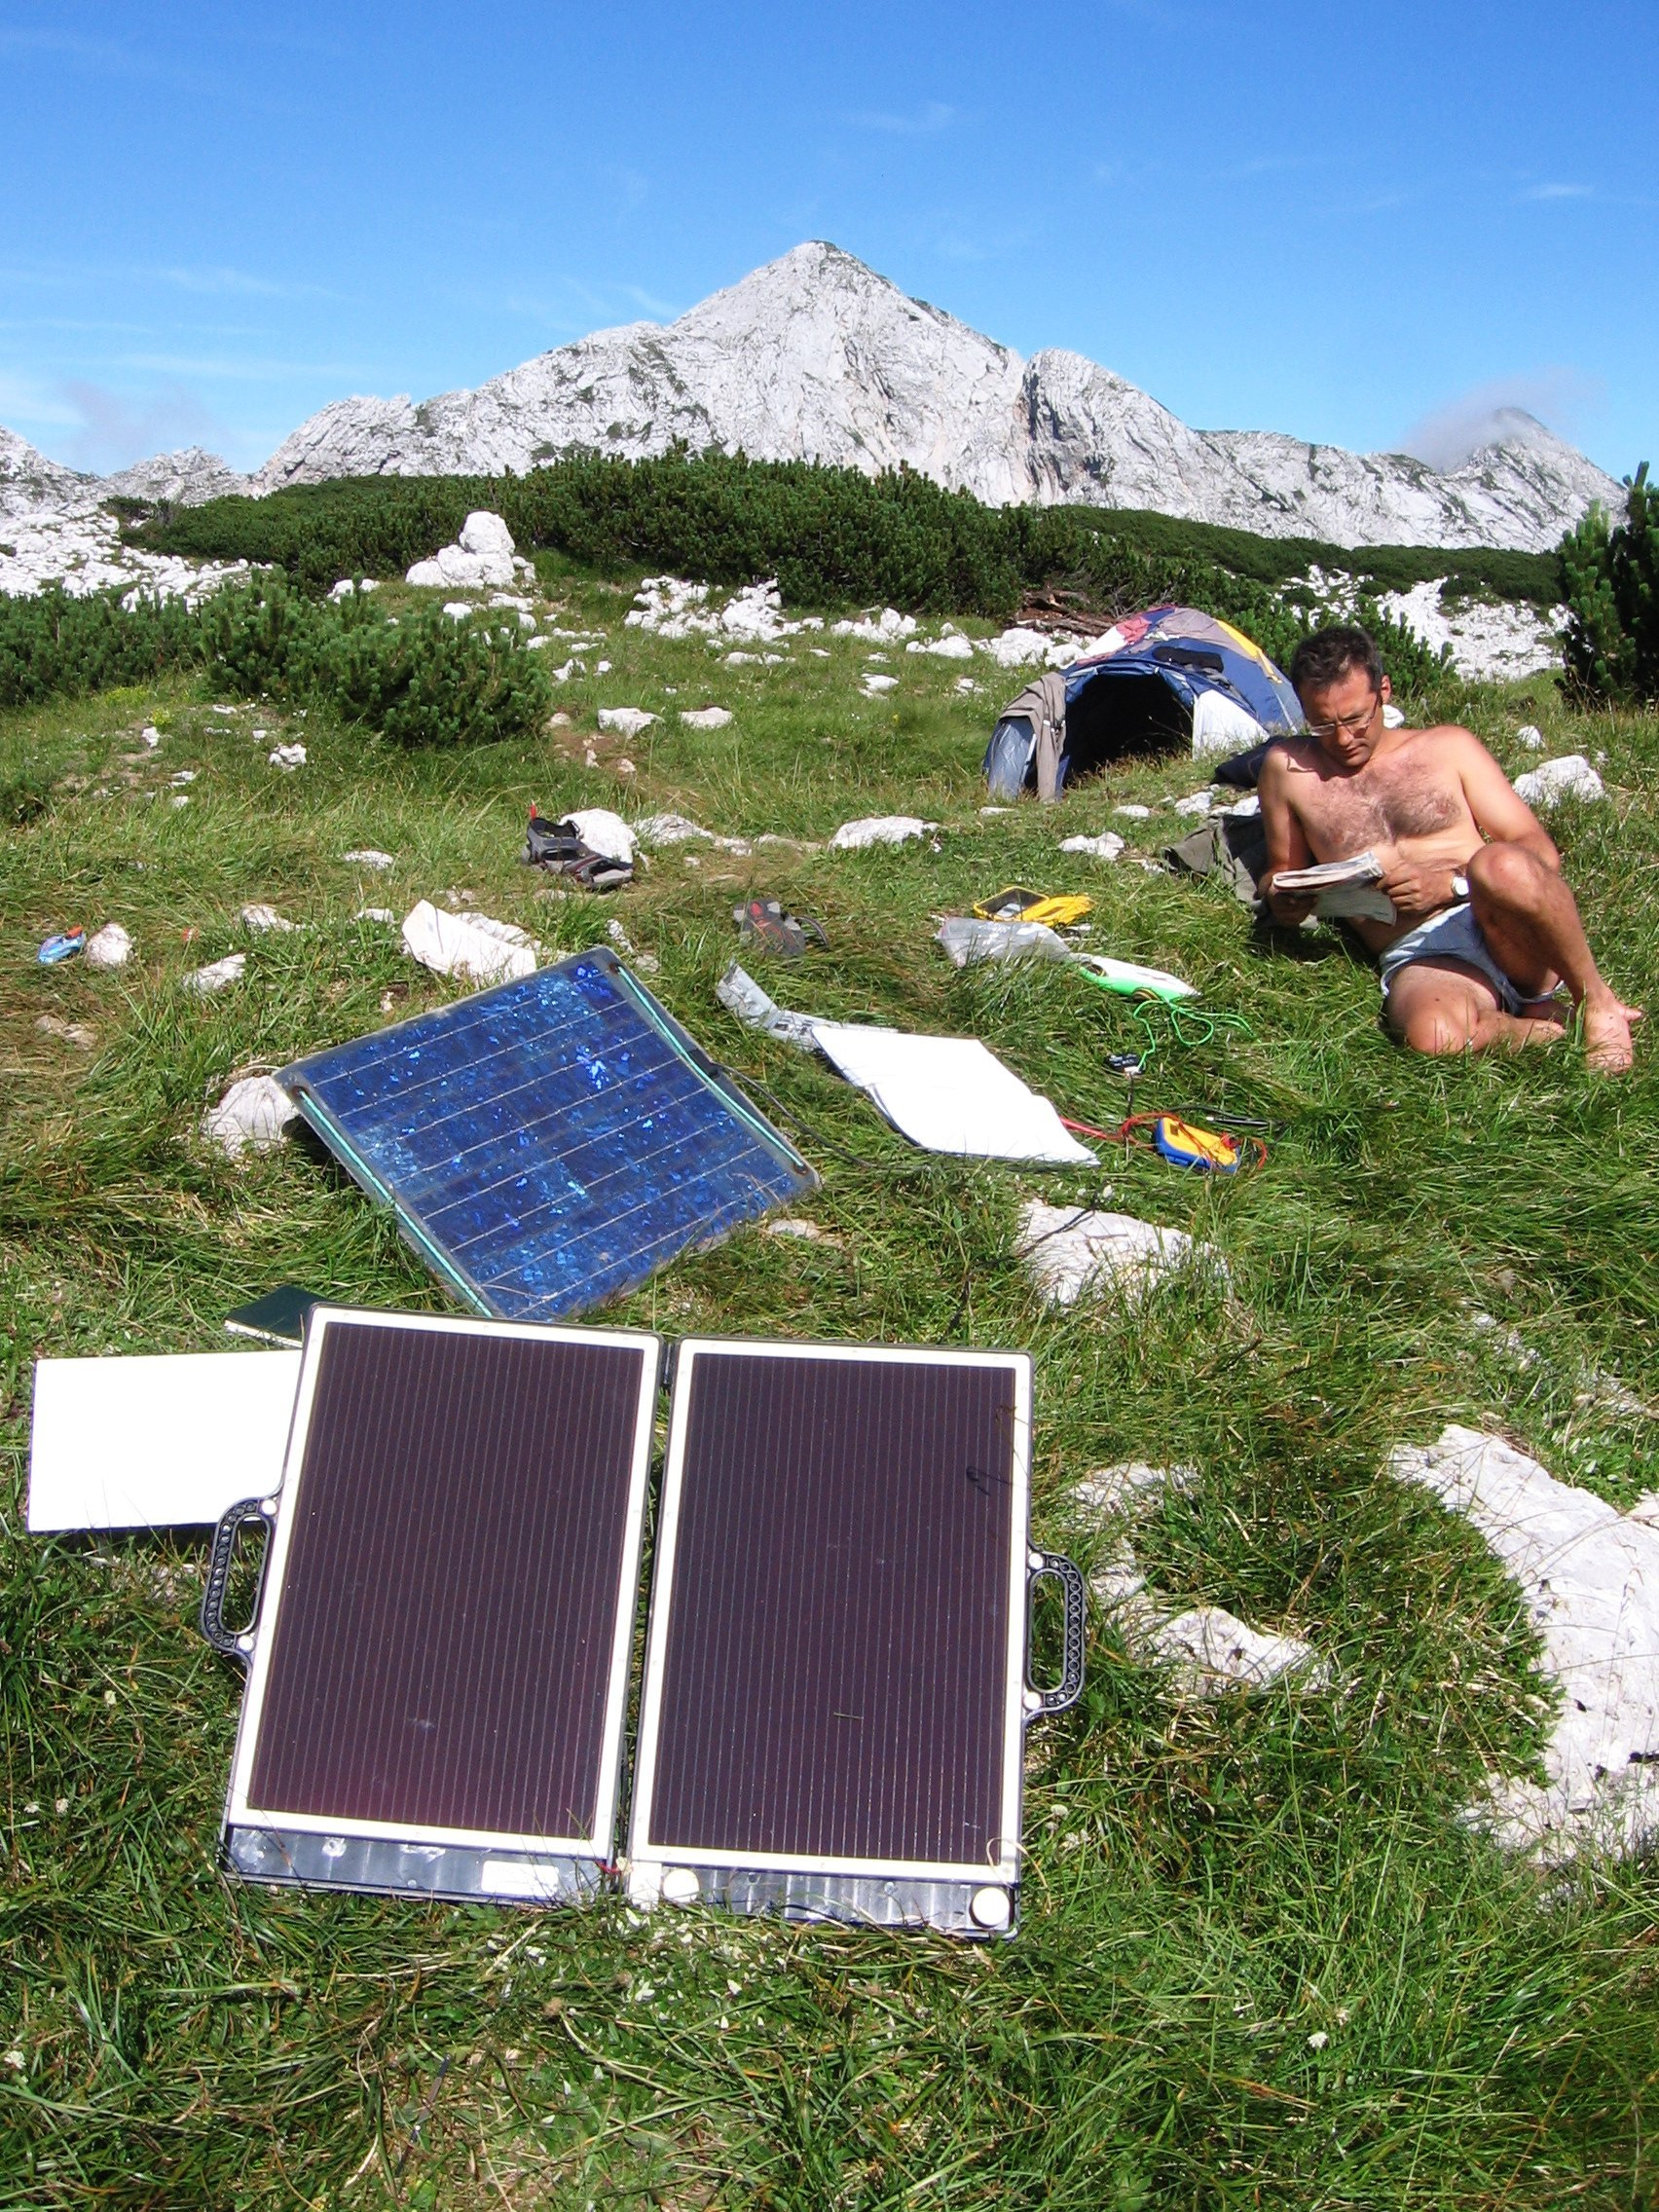
\includegraphics[height=\paperheight]{2008/outro/Jarvist Frost - canon a520 - both solar panels with skrbina in the background--orig.jpg}
 					}
	}
\BgThispage
